%%%%%%%%%%%%%%%%%%%%%%%%%%%%%%%%%%%%%%%%%%%%%%%%%%%%%%%%%%%%%%%%%
% Dissertacao de Mestrado / Dept Fisica, CFM, UFSC              %
% Andre@UFSC - 2011                                             %
%%%%%%%%%%%%%%%%%%%%%%%%%%%%%%%%%%%%%%%%%%%%%%%%%%%%%%%%%%%%%%%%%


%:::::::::::::::::::::::::::::::::::::::::::::::::::::::::::::::%
%                                                               %
%                          Capítulo 4                           %
%                                                               %
%:::::::::::::::::::::::::::::::::::::::::::::::::::::::::::::::%

%***************************************************************%
%                                                               %
%                    Problemas astrofísicos                     %
%                                                               %
%***************************************************************%

\chapter{Problemas astrofísicos}
\label{sec:Problemas}

% TODO: Comentar sobre \citet{Chilingarian2011}.
TODO: Comentar sobre \citet{Chilingarian2011}. Como fica UV no diagrama
$g-r$ contra $NUV-r$?

% TODO: Classificação das galáxias com o WHAN \citep{CidFernandes2011}.
TODO: Classificação das galáxias com o WHAN \citep{CidFernandes2011}. Ver também
o BPT \citep{CidFernandes2010}.

% TODO: Classes de galáxias no diagrama cor-cor UV
TODO: Classes de galáxias no diagrama $g-r$ contra $NUV-r$. Notar que existe uma
sequência.

% TODO: Parâmetros físicos das galáxias no diagrama de cores.
TODO: Parâmetros físicos das galáxias no diagrama de cores.

% TODO: Falar da sequência evolutiva das classes.
TODO: Falar da sequência evolutiva das classes.

% TODO: Comentar sobre: (Retired != passivas) == legal!
TODO: Comentar sobre: (Retired != passivas) == legal!

\begin{figure}
	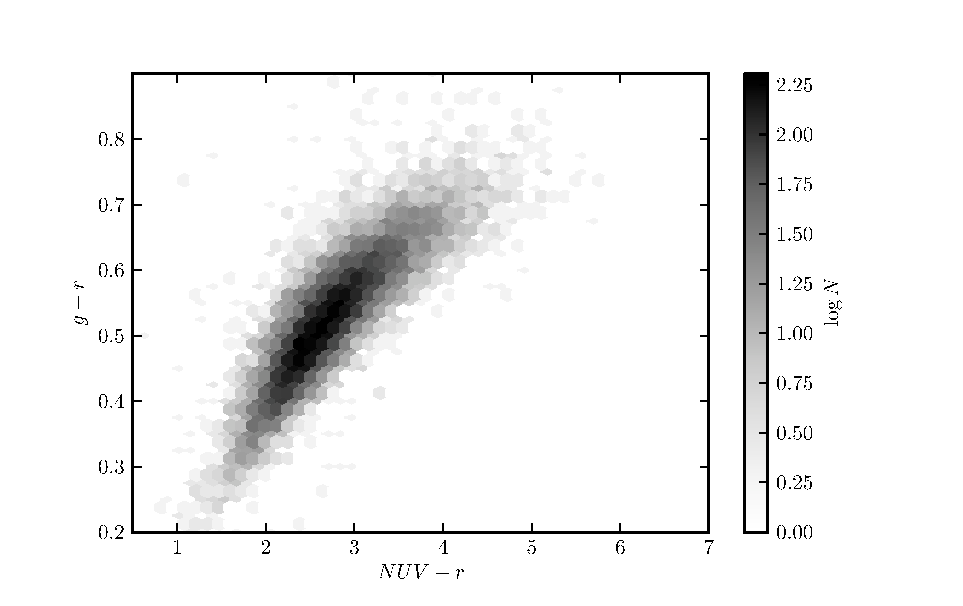
\includegraphics{figuras/uvcolor-color-density.eps}
	\caption[Densidade de galáxias no diagrama cor--cor UV.]
	{Densidade de galáxias em função de cor UV ($NUV-r$) e cor óptica ($g-r$). A
	intensidade dos bins hexagonais é o logaritmo do número de pontos dentro do
	bin, para melhorar a visualização. Foram selecionados objetos da amostra do
	\starlight com magnitude na banda $z$ entre $-23$ e $-21,5$ e {\em redshift}
	entre $0,04$ e $0,17$. As magnitudes $g$, $r$ e $z$ são do \SDSS.}
	\label{fig:DensityColor}
\end{figure}

\begin{figure}
	\includegraphics{figuras/uvcolor-color.eps}
	\caption[Diagrama cor--cor UV para os diversos parâmetros \starlight.]
	{Parâmetros físicos das galáxias em função de cor UV e cor óptica. Foi
	utilizada a mesma amostra da figura \ref{fig:DensityColor}. O contorno
	das figuras representam os níveis referentes à figura \ref{fig:DensityColor}.
	As cores dos pontos nos painéis correspondem a: {\bf (a)} Logaritmo da idade
	média da galáxia, ponderada pelo fluxo das SSP componentes. {\bf (b)} O mesmo
	que a anterior, mas ponderada pela massa das SSP. {\bf (c)} Metalicidade média
	da galáxia ponderada pelo fluxo das SSP cmponentes. {\bf (d)} O mesmo que a
	anterior, ponderada pela massa das SSP. {\bf (e)} Logaritmo da massa estelar da
	galáxia, em massas solares. {\bf (f)} Extinção por poeira na galáxia, na banda
	V.}
	\label{fig:ColorStarlightParam}
\end{figure}

\begin{figure}
	\includegraphics{figuras/whan.eps}
	\caption[Diagrama de diagnóstico WHAN.]
	{Diagrama de diagnóstico WHAN. As linhas tracejadas separam as galáxias
	em classes. {\bf Azul}: galáxias de formação estelar (SF). {\bf Verde
	claro}: galáxias com núcleo ativo forte (sAGN). {\bf Verde forte}:
	galáxias com núcleo ativo fraco (wAGN). {\bf Preto}: galáxias aposentadas
	(RG). {\bf Vermelho}: galáxias passivas. {\bf Magenta}: Galáxias que não se
	encaixam em nenhuma destas classes.}
	\label{fig:Whan}
\end{figure}

\begin{figure}
	\includegraphics{figuras/whan-uv.eps}
	\caption[Cores ultravioleta no diagrama WHAN.]
	{Diagrama WHAN semelhante ao da figura \ref{fig:Whan}. A cor dos pontos
	representa $NUV-r$. Galáxias de formação estelar são mais azuis do que
	as passivas.}
	\label{fig:WhanUV}
\end{figure}

\begin{figure}
	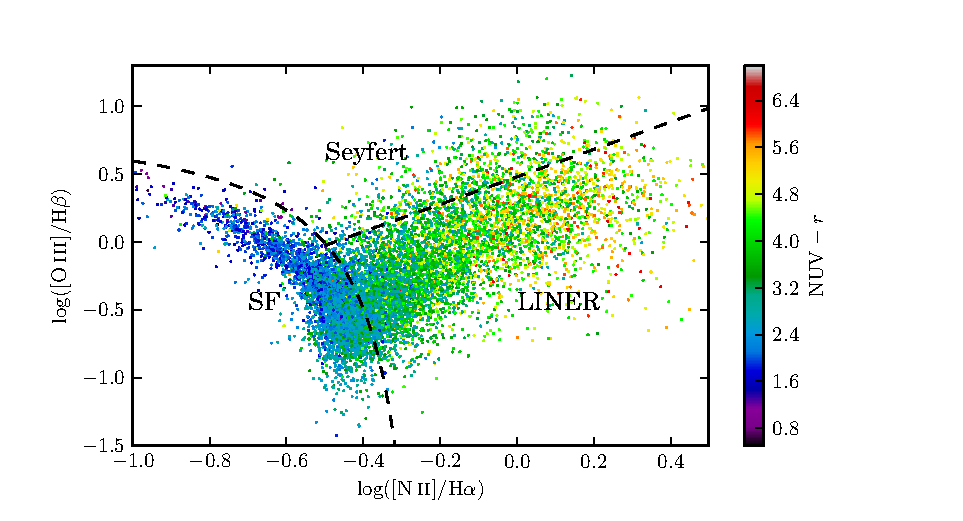
\includegraphics{figuras/bpt-uv.eps}
	\caption[Cores ultravioleta no diagrama BPT.]
	{Diagrama BPT, também usado para classificar galáxias. A cor dos
	pontos representa $NUV-r$. As linhas tracejadas mostram a separação das
	classes conforme \citet{CidFernandes2010}.}
	\label{fig:BPTUV}
\end{figure}

\begin{figure}
	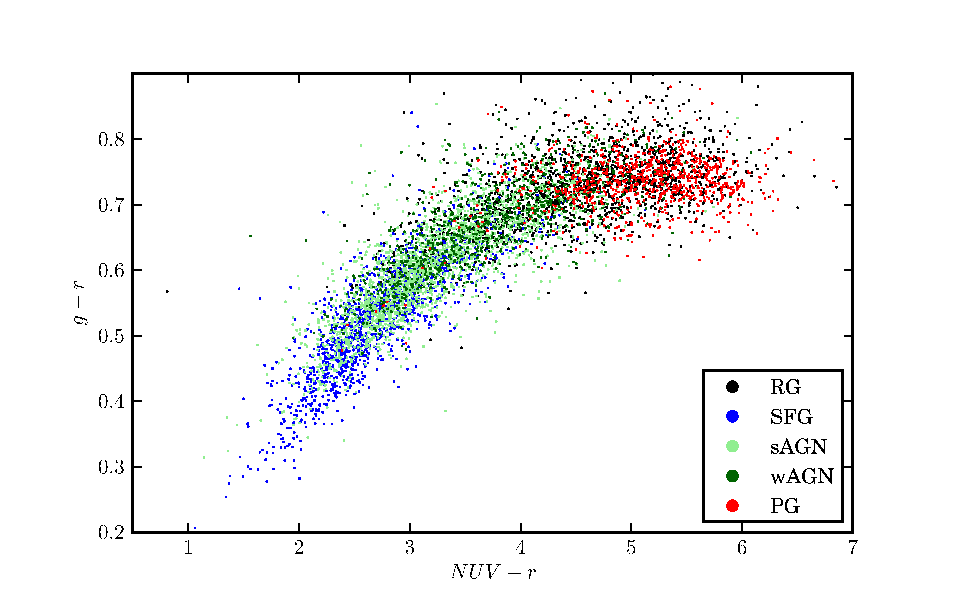
\includegraphics{figuras/uvcolor-color-class.eps}
	\caption[Diagrama cor--cor UV de acordo com o tipo de galáxia.]
	{Classes de galáxias no diagrama cor--cor UV. As cores referentes às classes de
	galáxia são as mesmas do diagrama WHAN (figura \ref{fig:Whan}). É possível
	notar uma separação entre as classes, embora não tão clara quanto no diagrama
	WHAN.}
	\label{fig:ColorClass}
\end{figure}

\begin{figure}
	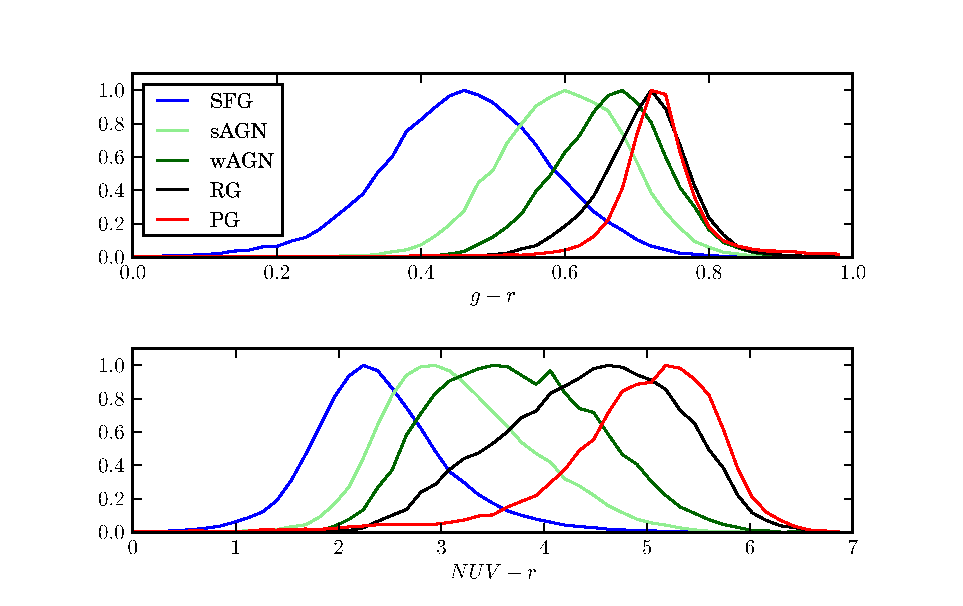
\includegraphics{figuras/histo_galtype_color.eps}
	\caption[Histogramas de cores para as classes de galáxias.]
	{Histogramas das cores óptica ($g-r$) e ultravioleta ($NUV-r$) para as
	classes de galáxias. A cor das linhas representa a classe conforme a figura
	\ref{fig:Whan}. Em ultravioleta a separação entre as classes de galáxias
	aposentadas (RG) e passivas (PG) torna-se mais clara. Note que os histogramas
	seguem o agrupamento das classes na figura \ref{fig:ColorClass}.}
	\label{fig:HistogramaCorClasse}
\end{figure}

\begin{figure}
	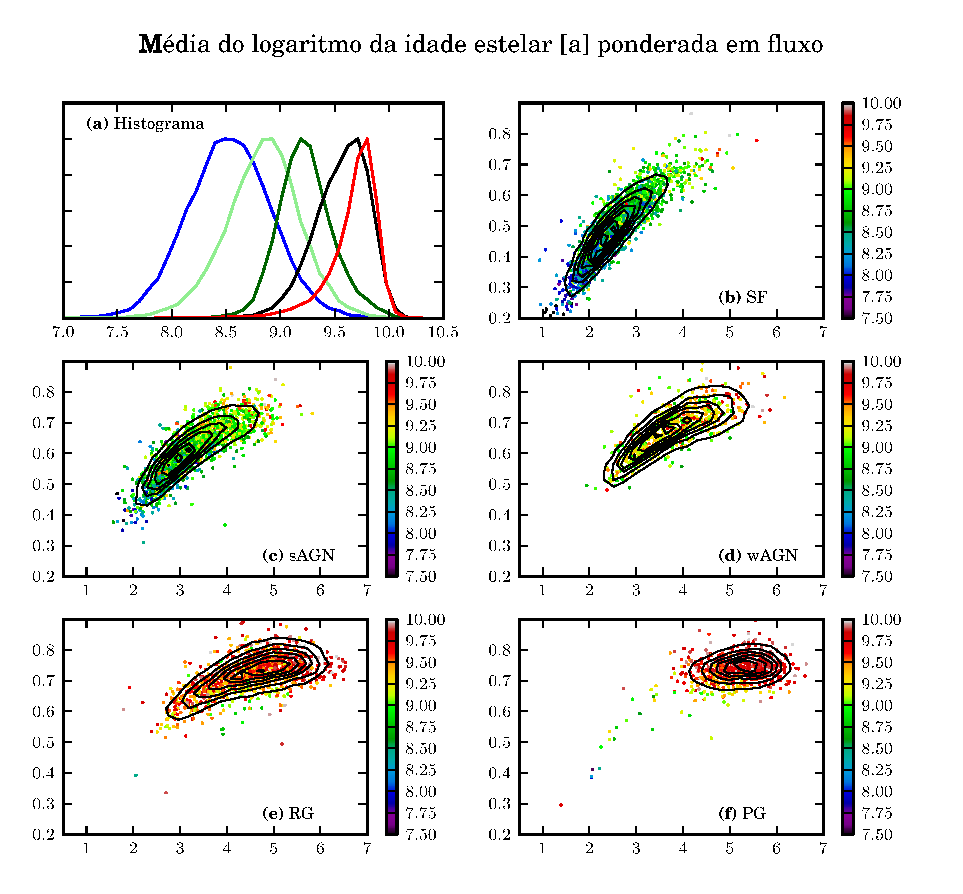
\includegraphics{figuras/uvcolor-color-at_flux-byclass.eps}
	\caption[Idade média das galáxias ponderada em fluxo no diagrama cor--cor UV.]
	{Idade média das galáxias ponderada em fluxo em função de $NUV-r$ e $g-r$. O
	painel {\bf (a)} contém todas as galáxias da amostra. Os painéis de {\bf (b)}
	a {\bf (f)} contém apenas as galáxias con formação estelar (SF), AGN fortes
	(sAGN), AGN fracas (wAGN), galáxias aposentadas (RG) e galáxias passivas (PG),
	respectivamente. Os contornos indicam a densidade de galáxias. A idade média da
	distribuição vai aumentando conforme a classe, na sequência apresentada.}
	\label{fig:ATFluxColor}
\end{figure}

\begin{figure}
	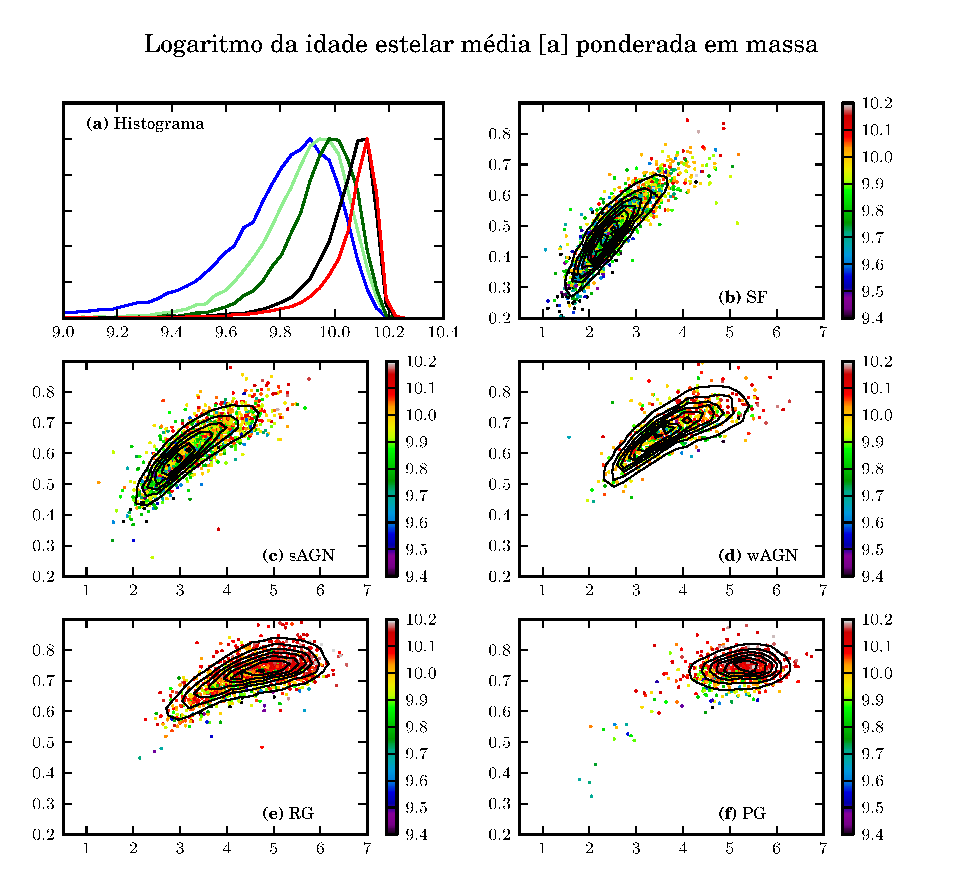
\includegraphics{figuras/uvcolor-color-at_mass-byclass.eps}
	\caption[Idade média das galáxias ponderada em massa no diagrama cor--cor UV.]
	{O mesmo que a figura \ref{fig:ATFluxColor}, para a idade média das galáxias
	ponderada pela massa das SSP componentes. Note que a escala de idades não é a
	mesma.}
	\label{fig:ATMassColor}
\end{figure}

\begin{figure}
	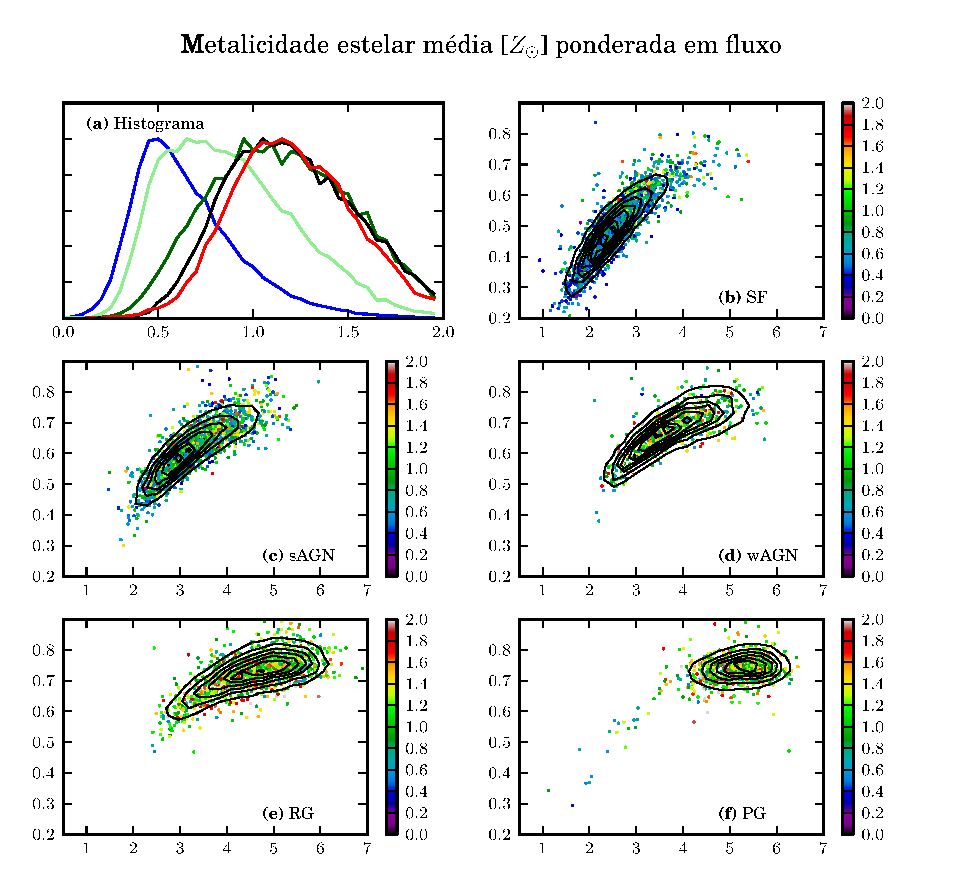
\includegraphics{figuras/uvcolor-color-am_flux-byclass.eps}
	\caption[Metalicidade das galáxias ponderada em fluxo no diagrama cor--cor UV.]
	{O mesmo que a figura \ref{fig:ATFluxColor}, para a metalicidade média das
	galáxias ponderada pelo fluxo das SSP componentes.}
	\label{fig:AMFluxColor}
\end{figure}

\begin{figure}
	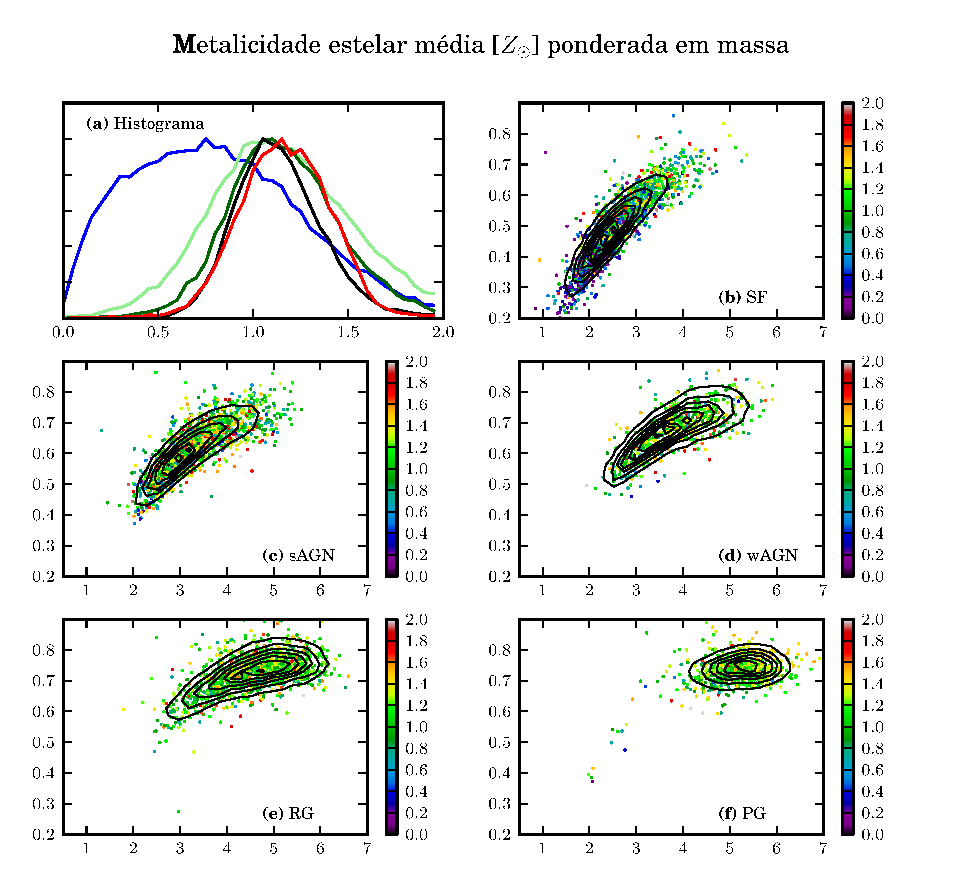
\includegraphics{figuras/uvcolor-color-am_mass-byclass.eps}
	\caption[Metalicidade das galáxias ponderada em massa no diagrama cor--cor UV.]
	{O mesmo que a figura \ref{fig:ATFluxColor}, para a metalicidade média das
	galáxias ponderada pelo massa das SSP componentes.}
	\label{fig:AMMassColor}
\end{figure}

\begin{figure}
	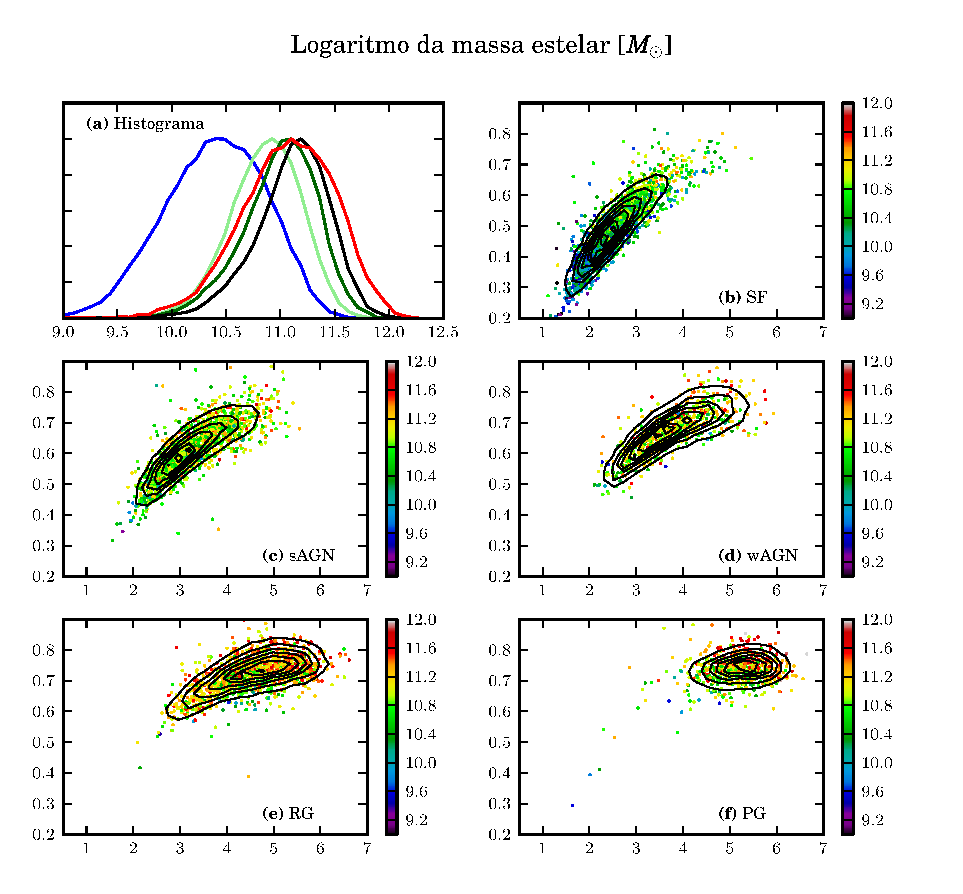
\includegraphics{figuras/uvcolor-color-mcor_gal-byclass.eps}
	\caption[Massa estelar das galáxias no diagrama cor--cor UV.]
	{O mesmo que a figura \ref{fig:ATFluxColor}, para o logaritmo da massa estelar
	das galáxias em massas solares.}
	\label{fig:MCorGalColor}
\end{figure}

\begin{figure}
	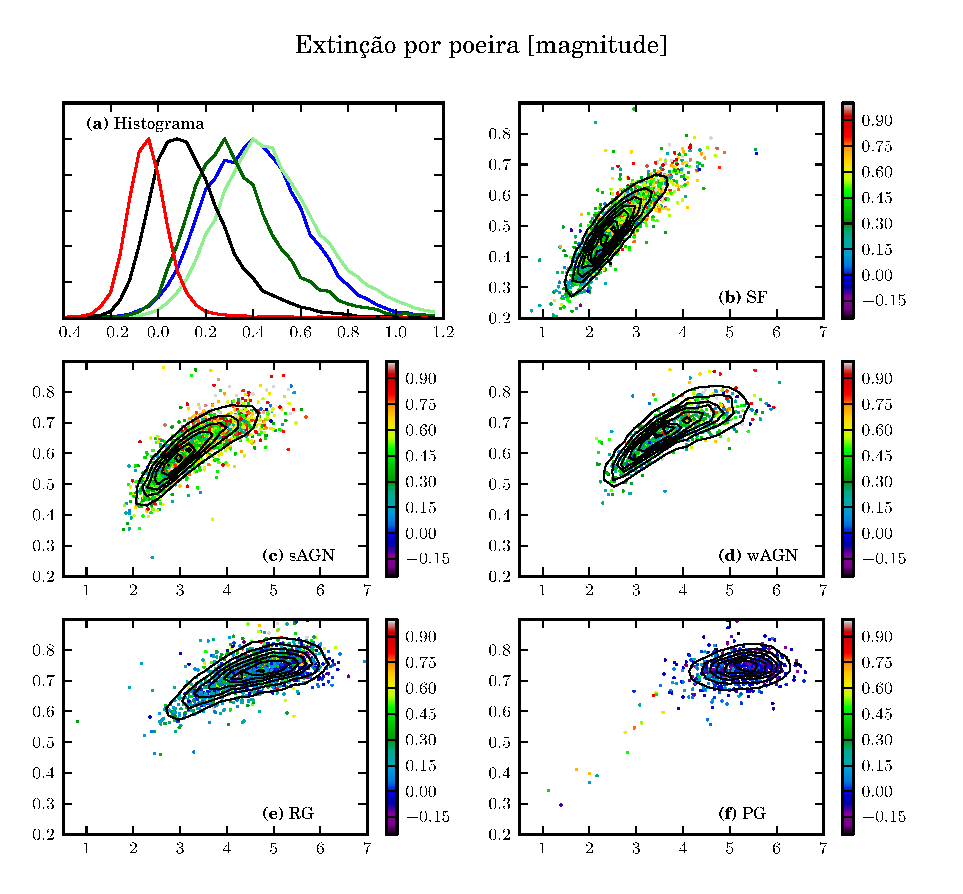
\includegraphics{figuras/uvcolor-color-AV-byclass.eps}
	\caption[Absorção por poeira no diagrama cor--cor UV.]
	{O mesmo que a figura \ref{fig:ATFluxColor}, para a extinção por
	poeira na banda V das galáxias.}
	\label{fig:AVColor}
\end{figure}

\begin{figure}
	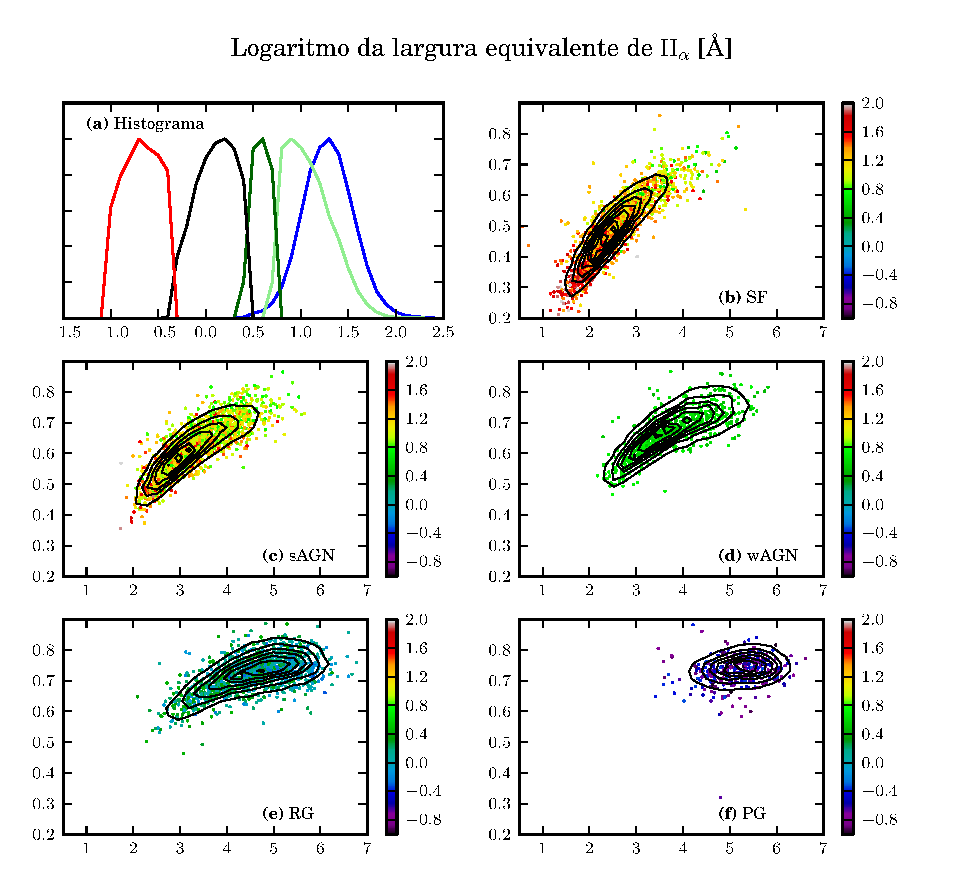
\includegraphics{figuras/uvcolor-color-halpha_ew-byclass.eps}
	\caption[Largura equivalente de $H_{\alpha}$ no diagrama cor--cor UV.]
	{O mesmo que a figura \ref{fig:ATFluxColor}, para o logaritmo da largura
	equivalente de $H_{\alpha}$ das galáxias.}
	\label{fig:EWHaColor}
\end{figure}



% End of this chapter
